% Chapter 4

% variables
\newcommand{\pdirfour}{chapters/plots/chapter4}

\chapter{Results} % Main chapter title

\label{chapter4} % For referencing the chapter elsewhere, use \ref{Chapter1}

In this chapter, we summarize the results of the NA64 experiment to this date, which include all the runs up to 2018, and are reported in detail in \cite{Banerjee:2020fue,Banerjee:2019hmi,NA64:2019imj,na64-prd,Banerjee:2018vgk,Banerjee:2016tad}. In the previous chapter, we did all the heavy lifting of estimating the background, calculating the systematic uncertainty, defining the selection criteria, and computing the signal yield. Now all is left to do is to un-blind the signal region and apply our selection criteria to the full sample, and simply count the number of events in the signal region that we defined. As the reader might already have guessed given no noble price has yet been awarded, no events was ever found in the signal region to this date. This leaves us with task of deciding how to exactly cast our results in a useful way, so that we are aware of what models are no longer a viable explanation to explain our cosmological measurements. This is done using the modified frequentist approach to compute the confidence level, taking the profile likelihood as test statistic in the asymptotic approximation \cite{Read_2002,JUNK1999435,Cowan:2010js}. This technique is summarized in Appendix.\ref{AppendixE}, and uses a representative data set provided by the Monte Carlo (also called Asimov data set) to obtain the median experimental sensitivity and its uncertainty.

To properly compare our results with all other experiment in the field, we chose the criteria of an 90\%C.L. as upper limit, and we exclude the hypothesis $\dmhypo$ accordingly. The standard way to show this result is a plot in the $dmplane$ showing the region were all hypothesis are excluded, combined with relevant results of other experiment and interesting region for a physicist to explore. The most relevant example in our case of relevant region is the one that explain the $\DMX$-anomaly as protophobic vector-boson \cite{PhysRevD.95.035017}. However, such way of presenting the results completely ignore other parameters that are interesting for the cosmological models. Indeed, since we always performed our experiment under the assumption that a decay channel dominates and the $\DM$ itself is not interacting, the exact mass of the LDM $m_{\chi}$ and the dark sector coupling $\alpha_D$ do not change the results of our experiment. Therefore, the results are presented using the standard variable:

\begin{equation}
  \label{eq:y-dm}
  y = \epsilon^2 \alpha_D (m_{\chi}/m_{\DM})^4
\end{equation}

This variables takes into account all relevant parameters for our model and scales with the cross-section for the freeze-out.

%----------------------------------------------------------------------------------------

\section{Invisible mode}
\label{ch4:sec:invis-mode}

No event has been recorded to date in the signal region defined as $E_{ECAL} < 50\gev;E_{HCAL}^{tot}<1\gev$. The results are shown in the $\dmplane$ in Fig.\

\begin{figure}[tbh!]
  \centering
  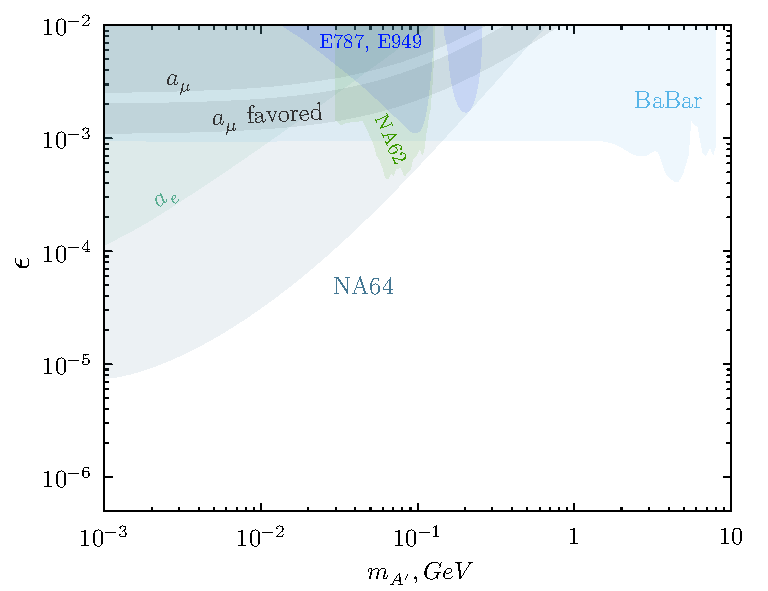
\includegraphics[width=0.45\textwidth,height=0.5\textwidth]{\pdirfour/exclusionInvisible.pdf}
  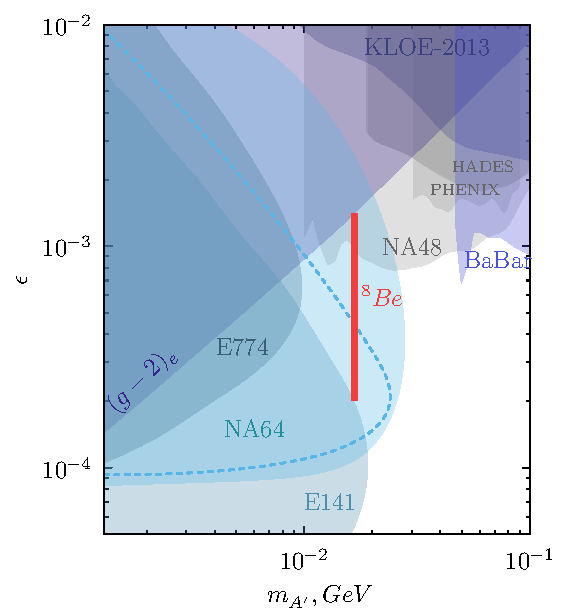
\includegraphics[width=0.45\textwidth,height=0.5\textwidth]{\pdirfour/exclusionVisible.pdf}
  \caption[Exclusion limits in the $\dmplane$]{The NA64 90\% exclusion region in the $\dmplane$ plane. The exclusion is shown for the data collected in the invisible mode setup (right) and visible mode setup (left), assuming the dominant decay is either invisible or visible respectively\cite{NA64:2019imj,Banerjee:2019hmi}. For the invisible mode, constraints from E787 and E949 \cite{PhysRevD.89.095006,Essig:2013vha},BABAR \cite{PhysRevLett.119.131804}, and recent NA62 results \cite{CortinaGil:2019nuo} are also shown, together with the muon $a_{\mu}$ favored area. For the visible mode, constraints from the experiments E774 \cite{PhysRevLett.67.2942}, E141 \cite{PhysRevLett.59.755}, BABAR \cite{babar1}, KLOE \cite{kloe2}, HADES \cite{hades}, PHENIX \cite{phenix}, NA48 \cite{na48} and bounds from the anomalous magnetic moment of the electron \cite{} are shown. A thick red line shows the full parameter space that can justify the $\DMX$-anomaly \cite{PhysRevD.95.035017}, $2 \times 10^{4} < \epsilon< 1.4 \times 10^{-3}$. Currently, the upper limit for the coupling is $\epsilon < 6.8 \times 10^{-4}$.}
  \label{fig:exclusion-inv}
\end{figure}

\section{Visible mode}
\label{ch4:sec:vis-mode}

%%% Local Variables:
%%% mode: latex
%%% TeX-master: "../PhDthesis"
%%% End:
